\documentclass[12pt, letterpaper]{article}

% --- PAQUETES ---
\usepackage[utf8]{inputenc}
\usepackage[T1]{fontenc}
\usepackage{lmodern}
\usepackage[spanish, es-tabla, es-nodecimaldot]{babel}
\usepackage[margin=2.5cm, headheight=30pt]{geometry}
\usepackage{amsmath, amsfonts, amssymb}
\usepackage{graphicx}
\usepackage{caption}
\usepackage{booktabs}
\usepackage{array}
\usepackage{tabularx}
\usepackage{fancyhdr}
\usepackage{enumitem}
\usepackage{microtype}
\usepackage{float}
\usepackage{xcolor}
\usepackage{listings}
\usepackage[american]{circuitikz}
\usepackage[spanish, ruled, linesnumbered]{algorithm2e}
\usepackage{hyperref}

\graphicspath{{img/}{logos/}}

% --- NOTACION ---
\newcommand{\pol}[2]{#1\angle {#2}^{\circ}}
\newcommand{\pendiente}[1]{\textcolor{red}{#1}}
\newcommand{\paso}[1]{\subsubsection*{#1}}
\setlength{\arraycolsep}{4pt}

% --- ESTILO DEL CODIGO ---
\definecolor{codegreen}{rgb}{0,0.5,0}
\definecolor{codegray}{rgb}{0.5,0.5,0.5}
\definecolor{codepurple}{rgb}{0.58,0,0.82}
\definecolor{backcolour}{rgb}{0.95,0.95,0.92}
\lstdefinestyle{pystyle}{
  language=Python,
  backgroundcolor=\color{backcolour},
  commentstyle=\color{codegreen},
  keywordstyle=\color{blue},
  numberstyle=\tiny\color{codegray},
  stringstyle=\color{codepurple},
  basicstyle=\ttfamily\footnotesize,
  breaklines=true,
  captionpos=b,
  keepspaces=true,
  numbers=left,
  numbersep=5pt,
  showstringspaces=false,
  tabsize=4
}
\lstdefinestyle{salida}{
  language={},
  backgroundcolor=\color{backcolour},
  basicstyle=\ttfamily\footnotesize,
  numbers=none,
  captionpos=b,
  keepspaces=true,
  columns=fixed
}
\lstset{style=pystyle}
\renewcommand{\lstlistingname}{Código}

% --- ENCABEZADO Y PIE ---
\pagestyle{fancy}
\fancyhf{}
\lhead{\textbf{Circuitos Eléctricos} \\ Métodos sistemáticos de análisis}
\rhead{\textbf{Equipo 6}, examen tipo A \\ Semestre 2027-1}
\cfoot{\thepage}
\renewcommand{\headrulewidth}{0.4pt}

\begin{document}

% ===================== PORTADA =====================
\begin{titlepage}
\begin{center}
    \noindent
    
\includegraphics[height=4.5cm]{Logo_UNAM.png}
    \hfill
    
\includegraphics[height=4.5cm]{Logo_FI.png}

    \vspace{1.8cm}
    {\Large \bfseries FACULTAD DE INGENIERÍA, UNAM}\\[0.6cm]
    {\large \bfseries CIRCUITOS ELÉCTRICOS}\\[0.6cm]
    {\large \bfseries MÉTODOS SISTEMÁTICOS DE ANÁLISIS\\[0.15cm] DE CIRCUITOS ELÉCTRICOS}\\[0.6cm]
    {\normalsize \bfseries EXAMEN TIPO A}\\[1.4cm]
\end{center}

\begin{center}
\begin{tabular}{ll}
\textbf{Asignatura:} & Circuitos Eléctricos \\[0.15cm]
\textbf{Equipo:} & 6 \\[0.15cm]
\textbf{Tipo de examen:} & A \\[0.15cm]
\textbf{Integrantes:} & Chávez López Brayan Alejandro \\
 & Daniel Kaleb Villanueva Figueroa \\
 & Enrique Hernandez Chanelo \\
 & Israel Raymundo Vázquez \\
 & Ortega Novoa Octavio \\[0.15cm]
\textbf{Semestre:} & 2027-1 \\
\end{tabular}
\end{center}
\end{titlepage}

% ===================== INTRODUCCION =====================
\section{Introducción}

En un circuito con varias mallas y varias fuentes, plantear las leyes de Kirchhoff una por una resulta largo y propenso
a errores de signo. Los métodos sistemáticos ordenan ese trabajo: el circuito se describe con unas cuantas matrices y
todas sus ecuaciones se obtienen al multiplicarlas. Como los pasos son siempre los mismos, se pueden programar. Hay un
método por nodos y otro por mallas; aquí se usa el de mallas.

\subsection{Fasores e impedancias}

Una fuente $A\cos(\omega t + \theta)$ se representa con su fasor $\pol{A}{\theta}$, con la amplitud pico. Si todas
las fuentes tienen la misma frecuencia $\omega$, cada elemento se cambia por su impedancia
\[
  Z_R = R, \qquad Z_L = j\omega L, \qquad Z_C = \frac{1}{j\omega C},
\]
y el circuito se resuelve como uno de corriente directa, pero con números complejos.

\subsection{Grafo y mallas}

Para plantear las ecuaciones solo importa cómo están conectados los elementos. El grafo guarda solo eso: cada nodo es
un punto y cada rama es una línea entre dos nodos. Cada rama lleva una flecha, que marca el sentido de su corriente
$J_k$; su voltaje $V_k$ es la caída de voltaje en ese mismo sentido.

Si el circuito tiene $n$ nodos y $b$ ramas, tiene
\[
  b - n + 1
\]
mallas independientes, que son las ventanas que se ven en el grafo. El contorno de afuera no se cuenta como malla,
porque su ecuación sale de sumar las de las ventanas.

\subsection{Rama genérica}

Todas las ramas se tratan igual. La rama genérica tiene una impedancia $Z_k$ en serie con una fuente de voltaje
$V_{sk}$, y las dos en paralelo con una fuente de corriente $J_{sk}$ (figura~\ref{fig:rama}). Si a una rama le falta
alguna fuente, esa fuente vale cero. Los elementos en serie se juntan en una rama, y una fuente de corriente que está en
paralelo con un elemento va en la rama de ese elemento.

\begin{figure}[H]
\centering
\begin{circuitikz}[scale=0.95, transform shape]
  \draw (0,0) node[circ]{} node[left]{nodo $i$}
        to[short, i=$J_k$] (1.5,0) -- (1.5,1.2)
        to[generic, l=$Z_k$] (4,1.2)
        to[V, l=$V_{sk}$] (6.5,1.2) -- (6.5,0)
        -- (8,0) node[circ]{} node[right]{nodo $j$};
  \draw (1.5,0) -- (1.5,-1.2) to[I, l_=$J_{sk}$] (6.5,-1.2) -- (6.5,0);
  \node at (0,-0.5) {$+$};
  \node at (8,-0.5) {$-$};
  \node at (4,-2.9) {$V_k$, caída de voltaje del nodo $i$ al nodo $j$};
\end{circuitikz}
\caption{Rama genérica $k$, que va del nodo $i$ al nodo $j$.}
\label{fig:rama}
\end{figure}

$V_{sk}$ es positiva si la flecha de la rama entra por su terminal $+$, y $J_{sk}$ es positiva si apunta en el mismo
sentido que la rama. Por la impedancia pasa $J_k - J_{sk}$, por lo que el voltaje de la rama es
\[
  V_k = V_{sk} + Z_k\,(J_k - J_{sk}) .
\]

\subsection{Ecuaciones de mallas en forma matricial}

El circuito se describe con estas matrices:
\begin{itemize}
  \item $M$, matriz de mallas, de $(b-n+1) \times b$, con un renglón por malla y una columna por rama. Cada elemento
        vale
        \[
          a_k = \begin{cases}
            \phantom{-}1 & \text{si la rama va en el mismo sentido que la malla,} \\
            -1 & \text{si va en sentido contrario,} \\
            \phantom{-}0 & \text{si la rama no es de esa malla.}
          \end{cases}
        \]
  \item $Z$, matriz de impedancias de rama, de $b \times b$. Es diagonal, con la impedancia $Z_k$ de cada rama.
  \item $V_{sk}$ y $J_{sk}$, vectores columna de $b \times 1$ con las fuentes de cada rama.
\end{itemize}

Con $M$, la ley de voltajes en todas las mallas y la relación entre corrientes de rama y de malla se escriben
\[
  M\,V_k = 0, \qquad\qquad J_k = M^T I_m ,
\]
donde $I_m$ es el vector de corrientes de malla. La segunda dice que por cada rama pasa la suma, con su signo, de las
corrientes de las mallas a las que pertenece. Al sustituir $V_k = V_{sk} + Z\,(J_k - J_{sk})$ y $J_k = M^T I_m$ en la
ley de voltajes se obtiene
\[
  M V_{sk} + M Z M^T I_m - M Z J_{sk} = 0
  \quad\Longrightarrow\quad
  \underbrace{M Z M^T}_{Z_m}\, I_m = \underbrace{M Z J_{sk} - M V_{sk}}_{E_{sm}} .
\]

\subsection{Procedimiento}
\label{sec:procedimiento}

De lo anterior se obtiene el procedimiento del método de mallas:
\begin{enumerate}
  \item Verificar que todas las fuentes independientes sean reales, es decir, que cada fuente de voltaje tenga un
        elemento en serie y cada fuente de corriente uno en paralelo. Si no, hacer la transformación que corresponda.
  \item Obtener los fasores de las fuentes y las impedancias de los elementos.
  \item Identificar los nodos, numerarlos y elegir el nodo de referencia.
  \item Obtener el grafo orientado y sus $b - n + 1$ mallas, todas en sentido horario.
  \item Obtener la matriz de mallas $M$.
  \item Obtener la matriz de impedancias de rama $Z$.
  \item Obtener los vectores de fuentes independientes $V_{sk}$ y $J_{sk}$.
  \item Calcular la matriz de impedancias de mallas, $Z_m = M\,Z\,M^T$.
  \item Calcular el vector de potenciales de fuentes independientes de mallas, $E_{sm} = M\,Z\,J_{sk} - M\,V_{sk}$.
  \item Calcular las corrientes de mallas, $I_m = Z_m^{-1}\,E_{sm}$.
  \item Calcular las corrientes de rama, $J_k = M^T\,I_m$.
  \item Calcular los voltajes de rama, $V_k = V_{sk} + Z\,J_k - Z\,J_{sk}$.
\end{enumerate}

Los pasos 1 a 7 consisten en interpretar el circuito y se hacen a mano. Sus resultados se le dan al programa como
datos, y el programa hace los pasos 8 a 12 y muestra cada matriz.

El objetivo de este trabajo es resolver por mallas los dos circuitos del examen con un programa propio, que hace los
pasos 8 a 12 y muestra cada matriz en el orden del procedimiento. El programa tiene además una interfaz gráfica, en la
que se pueden cambiar los valores de los elementos y de las fuentes y resolver de nuevo.

% ===================== HOJA DEL EXAMEN =====================
\clearpage
\section{Hoja del examen}

\begin{figure}[H]
\centering
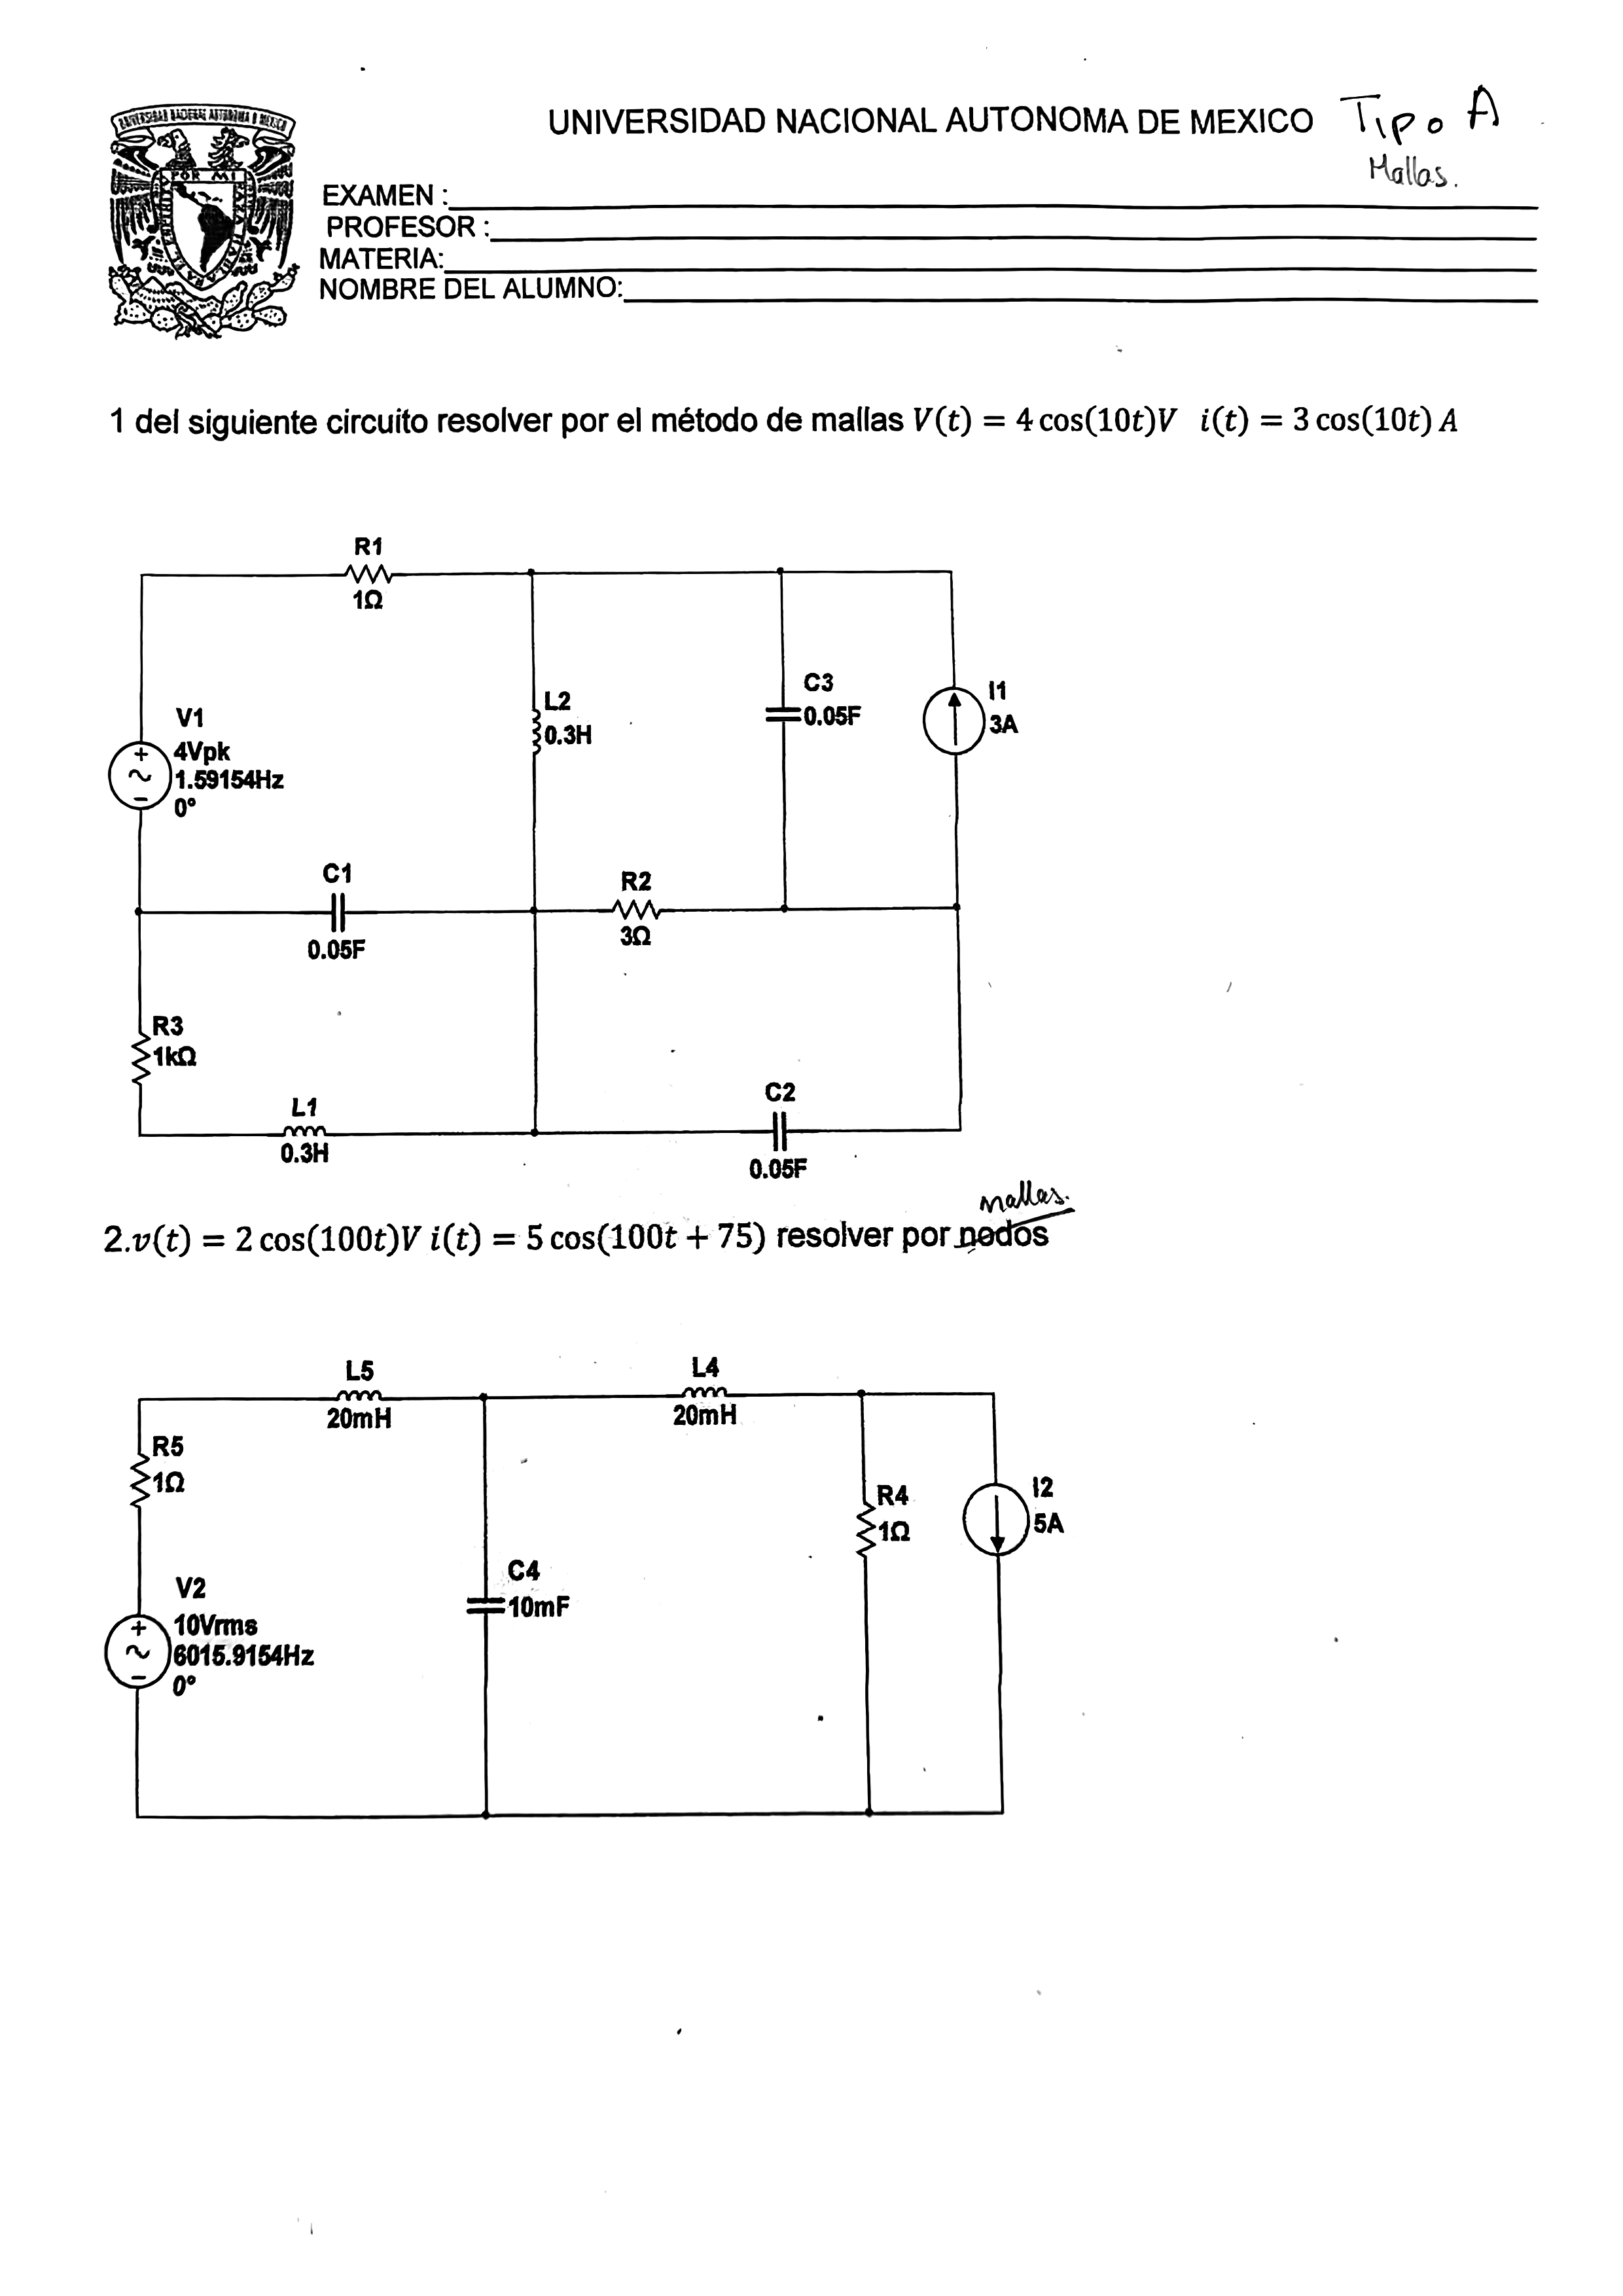
\includegraphics[height=0.82\textheight]{examen_tipoA.png}
\caption{Hoja del examen.}
\label{fig:examen}
\end{figure}

% ===================== PROGRAMA =====================
\clearpage
\section{Programa}

El programa resuelve por mallas los dos circuitos del examen. Recibe los valores de los elementos, la amplitud pico y
la fase de cada fuente y una frecuencia por circuito, en hertz. Entrega las corrientes de malla $I_m$, las corrientes de
rama $J_k$ y los voltajes de rama $V_k$, junto con todas las matrices en el orden del procedimiento ($Z$, $V_{sk}$,
$J_{sk}$, $M$, $M^T$, $Z_m$, $E_{sm}$, $I_m$, $J_k$ y $V_k$) y el dibujo del grafo de cada circuito. La forma de los
circuitos y la matriz $M$ son fijas; lo que se puede cambiar son los valores.

Está escrito en Python y usa numpy para las matrices, matplotlib para dibujar los grafos y tkinter con Pillow para la
interfaz. Hay tres formas de usarlo, desde la carpeta principal del repositorio:
\begin{itemize}
  \item \texttt{python codigo/interfaz.py} abre la interfaz gráfica;
  \item el ejecutable \texttt{Mallas\_Equipo6.exe} abre la misma interfaz y no necesita Python;
  \item \texttt{python codigo/mallas.py} resuelve los dos circuitos con los valores del examen, imprime las matrices
        en la terminal y guarda el dibujo de cada grafo en \texttt{reporte/img/}.
\end{itemize}
El código está repartido en cinco archivos (tabla~\ref{tab:archivos}).

\begin{table}[H]
\centering
\caption{Archivos del programa.}
\label{tab:archivos}
\begin{tabularx}{\textwidth}{lX}
\toprule
Archivo & Qué tiene \\
\midrule
\texttt{codigo/circuitos.py} & Los datos de los dos circuitos: los valores del examen, la matriz $M$, una función
que arma las ramas con cualquier juego de valores y la posición de cada nodo y malla en el dibujo. \\
\texttt{codigo/mallas.py} & El método. Revisa $M$, arma las matrices, hace los pasos 8 a 12 e imprime los
resultados. Al correrlo solo, resuelve los dos circuitos con los valores del examen. \\
\texttt{codigo/grafo.py} & El dibujo del grafo de cada circuito. \\
\texttt{codigo/interfaz.py} & La interfaz gráfica: portada y una pantalla por circuito con los valores y los
resultados. \\
\texttt{codigo/crear\_ejecutable.ps1} & Crea el ejecutable de la interfaz con PyInstaller. \\
\bottomrule
\end{tabularx}
\end{table}

\subsection{Datos de cada circuito}

Cada circuito tiene en \texttt{circuitos.py} un diccionario con los valores del examen, su matriz $M$ y una función que
arma sus ramas. Los valores van en unidades básicas: ohms, henrys, farads, volts, amperes, grados y hertz. La función
\texttt{armarCircuito1} recibe un diccionario de valores, sea el del examen o uno leído en la interfaz, calcula
$\omega = 2\pi f$, los fasores de las fuentes con \texttt{fasor} y las impedancias con \texttt{inductor} y
\texttt{capacitor}. Cada rama es una tupla con el nodo del que sale, el nodo al que entra, su impedancia, $V_{sk}$,
$J_{sk}$ y el nombre de sus elementos. La matriz $M$ se escribe a mano a partir del grafo y no depende de los valores.
El código~\ref{cod:datos1} tiene los datos del circuito 1; la función devuelve además las ramas, $M$ y los datos del
dibujo en un diccionario.

\lstinputlisting[linerange={7-17,20-54}, caption={Funciones de impedancia y de fasor y datos del circuito 1 en
\texttt{codigo/circuitos.py}.}, label={cod:datos1}]{../codigo/circuitos.py}

\subsection{Revisión de la matriz de mallas}

Como $M$ se escribe a mano, un signo equivocado daría resultados falsos sin ningún aviso. Por eso, antes de resolver,
la función \texttt{revisarMallas} arma la matriz de incidencia $A$ con los nodos de cada rama, con $+1$ en el nodo del
que sale y $-1$ en el que entra. Cada malla es un lazo cerrado, así que en todos los nodos la corriente que entra por
sus ramas es la que sale, y eso se escribe $M A^T = 0$. También revisa que $M$ tenga $b - n + 1$ renglones
independientes. Si algo falla, el programa se detiene con un mensaje de error (código~\ref{cod:revisar}).

\begin{lstlisting}[caption={Función \texttt{revisarMallas} de \texttt{codigo/mallas.py}.}, label={cod:revisar}]
def revisarMallas(ramas, matrizMallas):
    # matriz de incidencia: renglon por nodo, columna por rama, 1 si la rama sale del nodo y -1 si entra
    nodos = sorted({rama[0] for rama in ramas} | {rama[1] for rama in ramas})
    A = np.zeros((len(nodos), len(ramas)))
    for k, rama in enumerate(ramas):
        A[nodos.index(rama[0]), k] = 1
        A[nodos.index(rama[1]), k] = -1

    # cada malla es un lazo, asi que sus ramas no pueden dejar corriente sobrando en ningun nodo
    M = np.array(matrizMallas, dtype=float)
    if not np.allclose(M @ A.T, 0):
        raise ValueError("la matriz de mallas no coincide con los nodos de las ramas")

    # tienen que ser b - n + 1 mallas independientes
    if M.shape[0] != len(ramas) - len(nodos) + 1 or np.linalg.matrix_rank(M) != M.shape[0]:
        raise ValueError("la matriz de mallas no tiene b - n + 1 mallas independientes")
\end{lstlisting}

\subsection{Cálculo}

La función \texttt{resolver} toma los datos de un circuito y arma $Z$, $V_{sk}$, $J_{sk}$ y $M$ como matrices de
numpy. Después hace los pasos 8 a 12 con las mismas fórmulas del procedimiento, una línea por paso
(código~\ref{cod:pasos}). Antes de invertir $Z_m$ revisa que tenga inversa, y al final devuelve $J_k$ y $V_k$, que la
interfaz usa para su tabla de resultados.

\begin{lstlisting}[caption={Matrices de entrada y pasos 8 a 12 en la función \texttt{resolver} de \texttt{codigo/mallas.py}.}, label={cod:pasos}]
impedancias = [complex(rama[2]) for rama in ramas]
Z = np.diag(impedancias)
Vsk = np.array([rama[3] for rama in ramas], dtype=complex)
Jsk = np.array([rama[4] for rama in ramas], dtype=complex)
M = np.array(circuito["matrizMallas"], dtype=complex)

# ecuaciones de mallas
Zm = M @ Z @ M.T
# si Zm casi no tiene inversa no hay solucion con esos valores, por ejemplo cuando
# un inductor y un capacitor se cancelan justo a esa frecuencia
if np.linalg.cond(Zm) > 1e12:
    raise ValueError("la matriz Zm no tiene inversa con estos valores")
Esm = M @ Z @ Jsk - M @ Vsk
Im = np.linalg.inv(Zm) @ Esm
Jk = M.T @ Im
Vk = Vsk + Z @ Jk - Z @ Jsk
\end{lstlisting}

numpy trabaja directamente con números complejos, así que las fórmulas se escriben casi igual que en papel.
\texttt{np.array} convierte una lista de Python en matriz o vector, y \texttt{np.diag} arma la matriz diagonal $Z$ con
la lista de impedancias. El operador \texttt{@} es el producto de matrices, \texttt{.T} da la transpuesta y
\texttt{np.linalg.inv} da la inversa de $Z_m$. \texttt{np.linalg.cond} da el número de condición de $Z_m$; si pasa de
$10^{12}$, la matriz prácticamente no tiene inversa y el programa se detiene con un mensaje. En \texttt{revisarMallas} se usan además \texttt{np.zeros}, que crea la
matriz $A$ llena de ceros, \texttt{np.allclose}, que revisa si $M A^T$ es cero, y \texttt{np.linalg.matrix\_rank}, que
cuenta cuántos renglones independientes tiene $M$.

\subsection{Salida}

Las matrices se imprimen en forma rectangular con \texttt{imprimirMatriz}, y los vectores con \texttt{imprimirPolar},
que pone cada valor en forma rectangular y polar. Para la forma polar, \texttt{np.abs} da la magnitud,
\texttt{np.angle} el ángulo y \texttt{np.degrees} lo pasa a grados. Cada renglón empieza con el número de rama o de
malla, y \texttt{/\_} es el símbolo de ángulo. Por ejemplo, el vector $E_{sm}$ del circuito 1 sale así:
\begin{lstlisting}[style=salida]
Esm = M Z Jsk - M Vsk, fuentes de malla
   1:      4.0000   +0.0000j   =       4.0000 /_     0.00 grados
   2:      0.0000   +6.0000j   =       6.0000 /_    90.00 grados
   3:      0.0000   +0.0000j   =       0.0000 /_     0.00 grados
   4:      0.0000   +0.0000j   =       0.0000 /_     0.00 grados
\end{lstlisting}

\subsection{Dibujo del grafo}

La función \texttt{figuraGrafo} de \texttt{codigo/grafo.py} dibuja el grafo con matplotlib, con los mismos datos de
las ramas y las posiciones de \texttt{circuitos.py}:
\begin{itemize}
  \item cada nodo es un círculo con su número;
  \item cada rama es una línea del nodo del que sale al nodo al que entra, con una flecha a la mitad y su nombre $b_k$;
  \item las ramas que unen los mismos dos nodos se dibujan curvas para que no se encimen, con una curva cuadrática;
  \item cada malla es una flecha circular roja en sentido horario con su nombre $M_k$;
  \item el nodo de referencia lleva el símbolo de tierra.
\end{itemize}
La función \texttt{dibujarGrafo} guarda esa figura como imagen en \texttt{reporte/img/}, y es la que aparece en el
paso 4 de cada circuito. En la interfaz, la misma figura se abre en otra ventana con el botón \emph{Ver grafo}.

\subsection{Interfaz}

La interfaz está hecha con tkinter, la biblioteca de ventanas que trae Python, y Pillow para cargar las imágenes. Al
abrirla aparece una portada con un botón para cada circuito (figura~\ref{fig:guiportada}).

\begin{figure}[H]
\centering
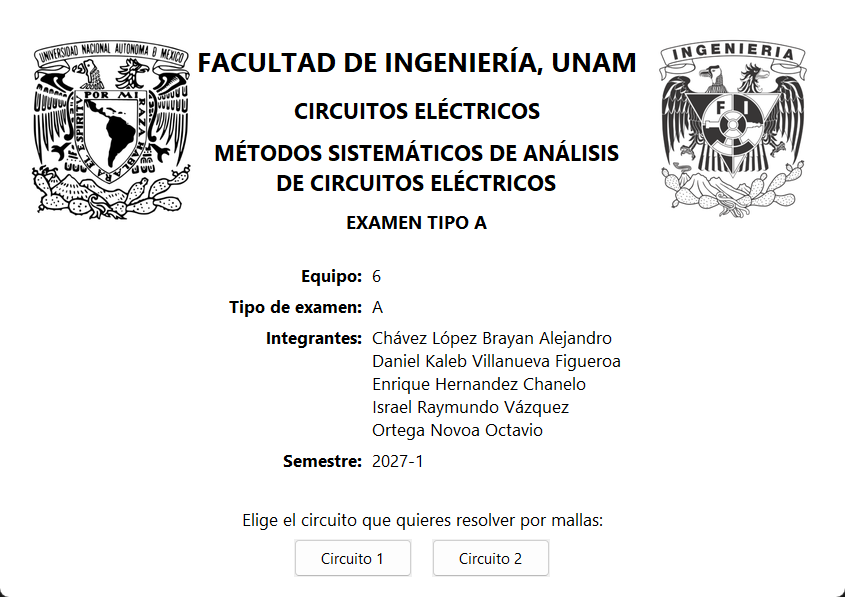
\includegraphics[width=0.6\textwidth]{gui_portada.png}
\caption{Portada de la interfaz.}
\label{fig:guiportada}
\end{figure}

Cada pantalla de circuito muestra el dibujo del examen con una casilla junto a cada elemento, donde se escribe su valor
y se elige la unidad: $\Omega$ o k$\Omega$, H o mH, F, mF o $\mu$F. Cada fuente tiene una casilla para su amplitud pico y
otra para su fase en grados, y la de voltaje lleva además la frecuencia del circuito. Al abrir la pantalla, las casillas
ya tienen los valores del examen, y el botón \emph{Valores del examen} los vuelve a poner
(figura~\ref{fig:guicircuito1}).

Las dos fuentes de un circuito comparten la frecuencia, porque los fasores e impedancias solo valen para una
frecuencia; por eso hay una sola casilla de frecuencia por circuito. Se pide en hertz, como en el dibujo del examen, y
el programa calcula $\omega = 2\pi f$. Con los valores del examen resulta $f = 10/2\pi = 1.591549$~Hz en el circuito 1
y $f = 100/2\pi = 15.915494$~Hz en el circuito 2.

\begin{figure}[H]
\centering
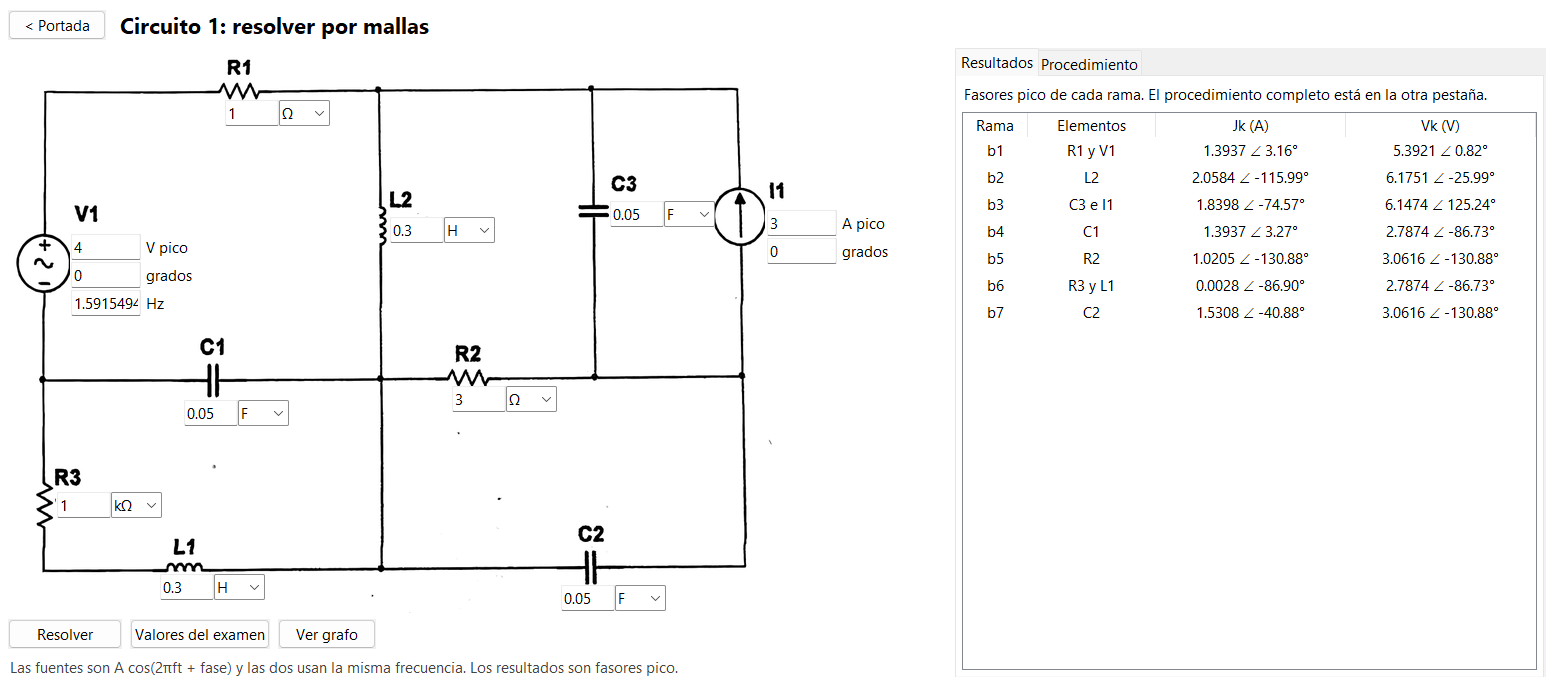
\includegraphics[width=\textwidth]{gui_circuito1.png}
\caption{Pantalla del circuito 1 con los valores del examen y sus resultados.}
\label{fig:guicircuito1}
\end{figure}

Con el botón \emph{Resolver}, la interfaz lee las casillas, pasa cada valor a unidades básicas y llama a
\texttt{armarCircuito1} o \texttt{armarCircuito2} con esos valores y después a \texttt{resolver}, la misma función de la
versión de terminal. Los fasores $J_k$ y $V_k$ de cada rama aparecen en forma polar en la pestaña \emph{Resultados}, y
todo lo que imprime \texttt{resolver} aparece en la pestaña \emph{Procedimiento} (figura~\ref{fig:guiprocedimiento}).
La figura~\ref{fig:guicircuito2} muestra la pantalla del circuito 2.

\begin{figure}[H]
\centering
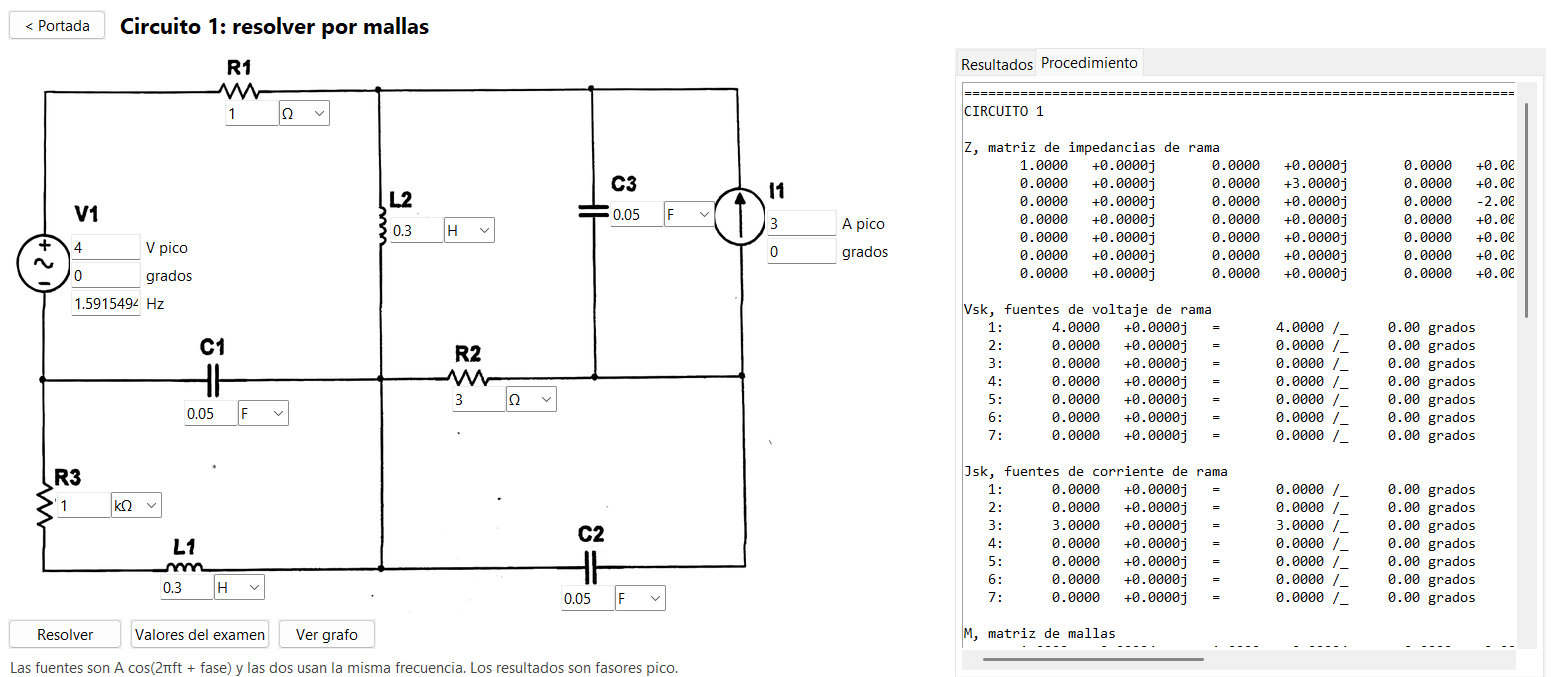
\includegraphics[width=\textwidth]{gui_procedimiento1.png}
\caption{Pestaña \emph{Procedimiento} del circuito 1.}
\label{fig:guiprocedimiento}
\end{figure}

\begin{figure}[H]
\centering
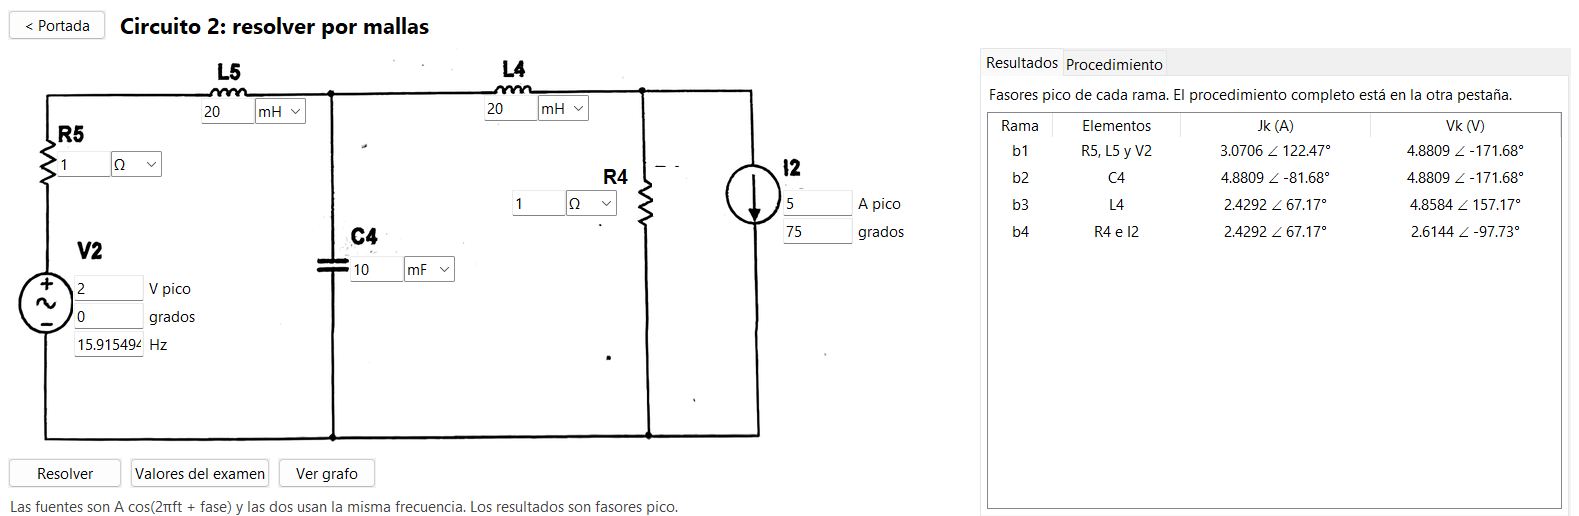
\includegraphics[width=\textwidth]{gui_circuito2.png}
\caption{Pantalla del circuito 2 con los valores del examen y sus resultados.}
\label{fig:guicircuito2}
\end{figure}

La interfaz no hace ningún cálculo del método. Solo lee valores y llama a las mismas funciones que la versión de
terminal, de modo que el código del método es el que se explica en esta sección y se puede revisar sin leer el de la
interfaz.

\subsection{Algoritmo}

El algoritmo~\ref{alg:flujo} resume lo que hace el programa al resolver un circuito desde la interfaz. En la versión de
terminal no se leen valores, porque usa los del examen, y el resto es igual.

\begin{algorithm}[H]
\caption{Flujo del programa al resolver un circuito.}
\label{alg:flujo}
\Entrada{valores de los elementos, amplitud y fase de cada fuente, frecuencia $f$}
\Salida{$I_m$, $J_k$, $V_k$, las matrices del procedimiento y el grafo}
Leer los valores de las casillas y pasarlos a unidades básicas\;
\lSSi{falta un valor, es negativo, o un capacitor o $f$ valen cero}{mostrar un mensaje y terminar}
Calcular $\omega = 2\pi f$, los fasores de las fuentes y las impedancias de las ramas\;
Armar $Z$, $V_{sk}$, $J_{sk}$ y $M$, y revisar $M$ contra la matriz de incidencia\;
$Z_m \leftarrow M Z M^T$\;
\lSSi{$Z_m$ no tiene inversa}{mostrar un mensaje y terminar}
$E_{sm} \leftarrow M Z J_{sk} - M V_{sk}$\;
$I_m \leftarrow Z_m^{-1} E_{sm}$, \quad $J_k \leftarrow M^T I_m$, \quad $V_k \leftarrow V_{sk} + Z J_k - Z J_{sk}$\;
Mostrar las matrices en el orden del procedimiento y la tabla de $J_k$ y $V_k$\;
Dibujar el grafo\;
\end{algorithm}

% ===================== CIRCUITO 1 =====================
\clearpage
\section{Circuito 1}

\subsection{Planteamiento del problema}

\begin{quote}
\emph{1. Del siguiente circuito resolver por el método de mallas $V(t) = 4\cos(10t)$~V, $i(t) = 3\cos(10t)$~A.}
\end{quote}

\begin{figure}[H]
\centering
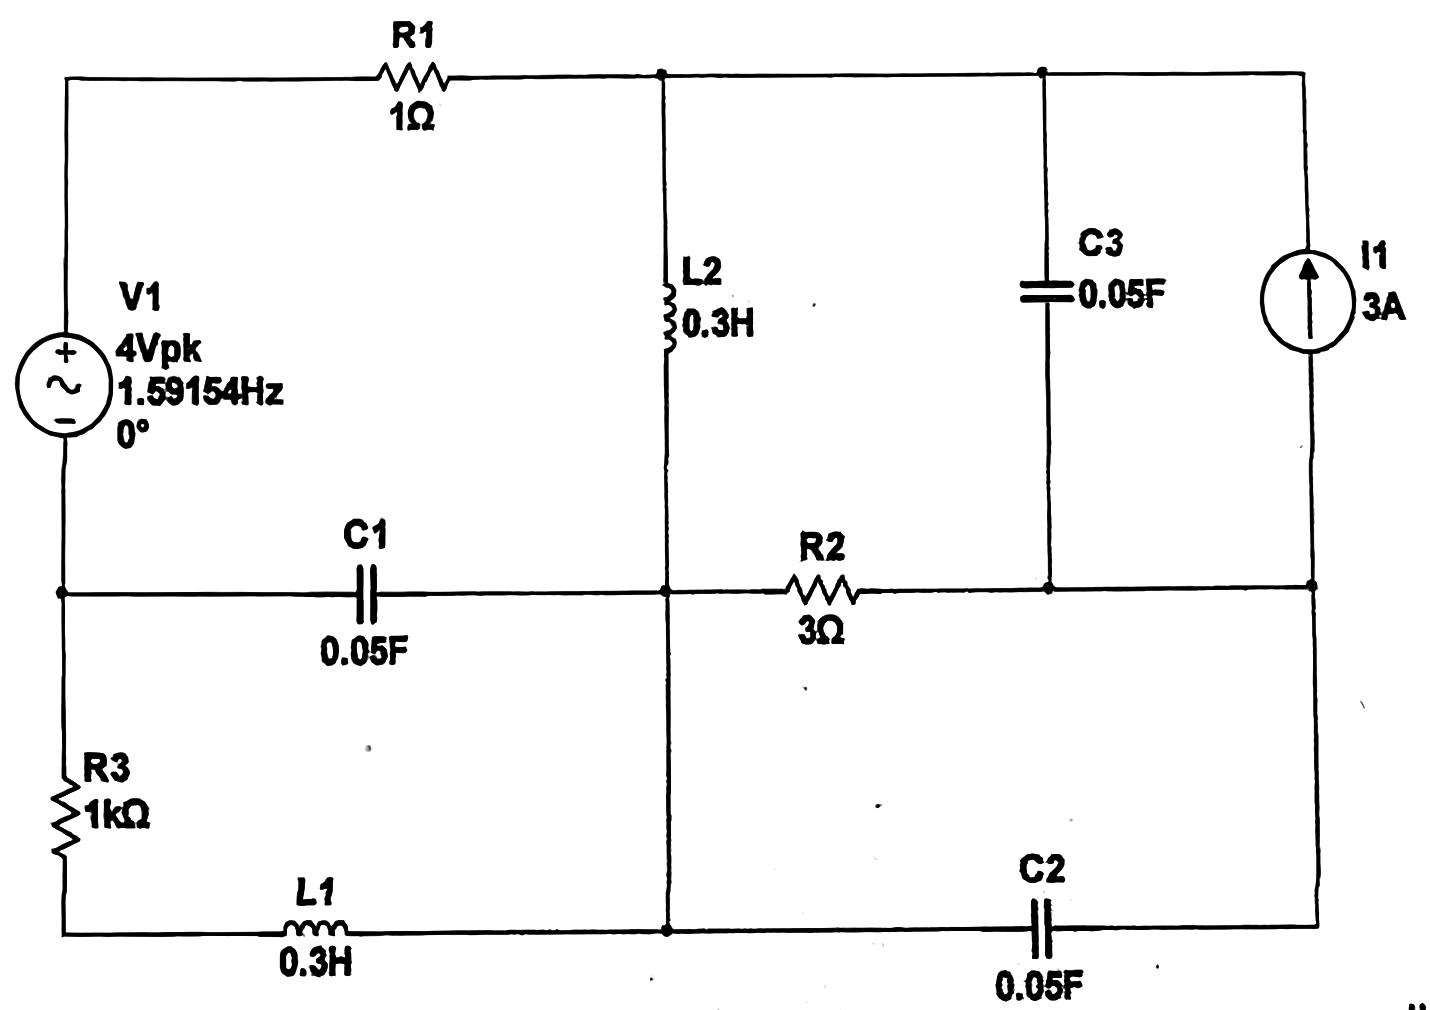
\includegraphics[width=0.78\textwidth]{circuito1.png}
\caption{Circuito 1.}
\label{fig:circuito1}
\end{figure}

Se buscan los fasores del voltaje $V_k$ y de la corriente $J_k$ de todas las ramas. Los elementos son
$R_1 = 1\,\Omega$, $R_2 = 3\,\Omega$, $R_3 = 1\,\text{k}\Omega$, $L_1 = L_2 = 0.3$~H y
$C_1 = C_2 = C_3 = 0.05$~F.

\subsection{Desarrollo}

\paso{1. Fuentes reales}

$V_1$ tiene a $R_1$ en serie e $I_1$ tiene a $C_3$ en paralelo, por lo que las dos fuentes son reales y no se
requiere ninguna transformación.

\paso{2. Fasores e impedancias}

Las dos fuentes tienen $\omega = 10$~rad/s, que es lo mismo que los 1.59154~Hz del dibujo, porque
$2\pi(1.59154) = 10$. Sus fasores son
\[
  V_1 = \pol{4}{0}\ \text{V}, \qquad I_1 = \pol{3}{0}\ \text{A},
\]
y las impedancias de los inductores y de los capacitores son
\[
  Z_{L} = j\omega L = j(10)(0.3) = j3\,\Omega, \qquad
  Z_{C} = \frac{1}{j\omega C} = \frac{1}{j(10)(0.05)} = \frac{1}{j0.5} = -j2\,\Omega.
\]

\paso{3. Nodos}

\begin{itemize}
  \item Nodo 1, arriba, donde se unen $R_1$, $L_2$, $C_3$ e $I_1$.
  \item Nodo 2, a la izquierda en medio, en la terminal $-$ de $V_1$, donde llegan $C_1$ y $R_3$.
  \item Nodo 3, al centro, donde se unen $L_2$, $C_1$, $R_2$ y el cable que baja hacia $L_1$ y $C_2$.
  \item Nodo 4, a la derecha en medio, donde se unen $C_3$, $I_1$, $R_2$ y el cable que baja hacia $C_2$. Es el nodo
        de referencia.
\end{itemize}

\paso{4. Grafo orientado y mallas}

$V_1$ va en una rama con $R_1$, $R_3$ en una con $L_1$, e $I_1$ en la rama de $C_3$. Resultan las siete ramas de la
tabla~\ref{tab:ramas1}, y con $b = 7$ y $n = 4$ hay
\[
  b - n + 1 = 7 - 4 + 1 = 4 \ \text{mallas}.
\]

\begin{table}[H]
\centering
\caption{Ramas del circuito 1.}
\label{tab:ramas1}
\begin{tabular}{cccccc}
\toprule
Rama & Sale $\to$ entra & Elementos & $Z_k$ ($\Omega$) & $V_{sk}$ (V) & $J_{sk}$ (A) \\
\midrule
$b_1$ & $1 \to 2$ & $R_1$ y $V_1$ & $1$ & $4$ & $0$ \\
$b_2$ & $1 \to 3$ & $L_2$ & $j3$ & $0$ & $0$ \\
$b_3$ & $4 \to 1$ & $C_3$ e $I_1$ & $-j2$ & $0$ & $3$ \\
$b_4$ & $2 \to 3$ & $C_1$ & $-j2$ & $0$ & $0$ \\
$b_5$ & $3 \to 4$ & $R_2$ & $3$ & $0$ & $0$ \\
$b_6$ & $2 \to 3$ & $R_3$ y $L_1$ & $1000 + j3$ & $0$ & $0$ \\
$b_7$ & $3 \to 4$ & $C_2$ & $-j2$ & $0$ & $0$ \\
\bottomrule
\end{tabular}
\end{table}

Las mallas van en sentido horario: $M_1 = \{b_1, b_2, b_4\}$ arriba a la izquierda, $M_2 = \{b_2, b_3, b_5\}$ arriba a
la derecha, $M_3 = \{b_4, b_6\}$ abajo a la izquierda y $M_4 = \{b_5, b_7\}$ abajo a la derecha
(figura~\ref{fig:grafo1}). Entre $C_3$ e $I_1$ no hay una ventana, porque los dos están en la rama $b_3$.

\begin{figure}[H]
\centering
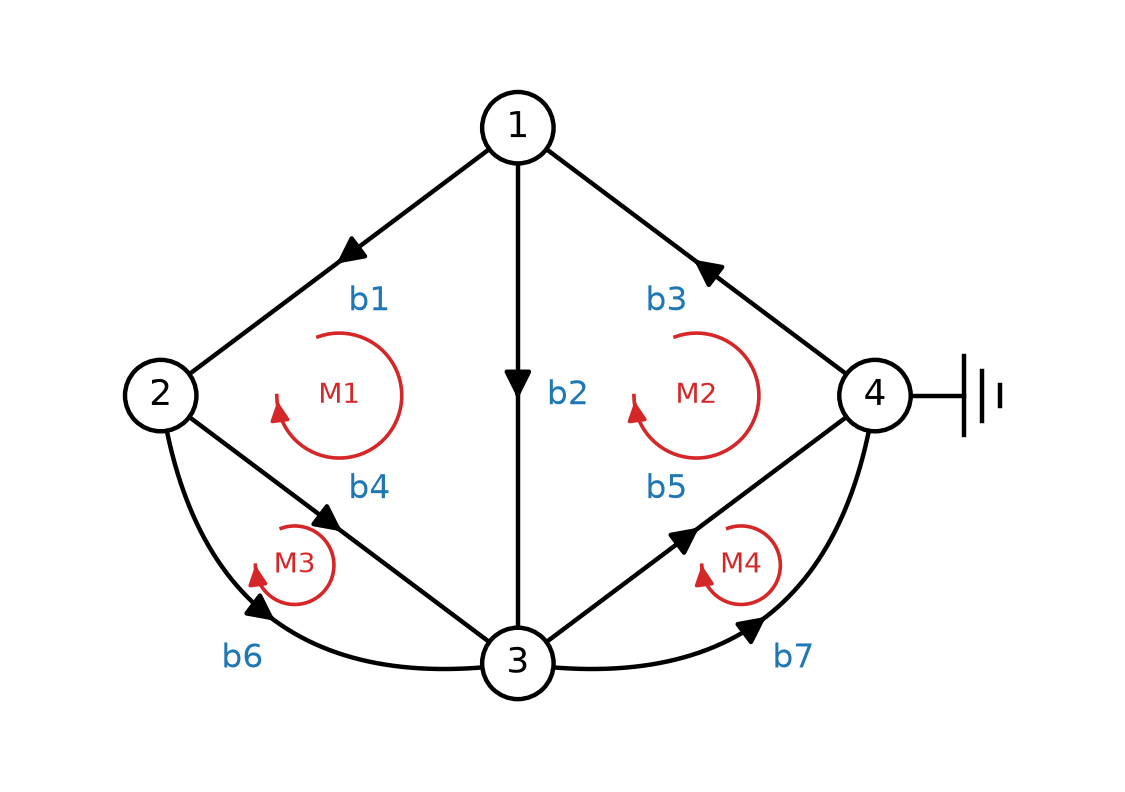
\includegraphics[width=0.72\textwidth]{grafo_circuito1.png}
\caption{Grafo orientado del circuito 1, dibujado por el programa.}
\label{fig:grafo1}
\end{figure}

\paso{5. Matriz de mallas}

Cada renglón de $M$ se llena recorriendo la malla en sentido horario. $M_1$ sube del nodo 2 al 1 por $b_1$, que va al
revés, baja del 1 al 3 por $b_2$, que va en el mismo sentido, y regresa del 3 al 2 por $b_4$, que va al revés. Su
renglón tiene $-1$, $1$ y $-1$ en esas columnas. Con las otras tres mallas se obtiene
\[
M = \begin{bmatrix}
 -1 &  1 &  0 & -1 &  0 &  0 &  0 \\
  0 & -1 & -1 &  0 & -1 &  0 &  0 \\
  0 &  0 &  0 &  1 &  0 & -1 &  0 \\
  0 &  0 &  0 &  0 &  1 &  0 & -1
\end{bmatrix}.
\]

\paso{6. Matriz de impedancias de rama}

\[
Z = \operatorname{diag}\left(1,\ j3,\ -j2,\ -j2,\ 3,\ 1000+j3,\ -j2\right)\ \Omega .
\]

\paso{7. Vectores de fuentes}

$b_1$ va del nodo 1 al 2 y entra a $V_1$ por su terminal $+$, por lo que $V_{s1} = 4$. $b_3$ va del nodo 4 al 1 y
la flecha de $I_1$ también sube, por lo que $J_{s3} = 3$:
\[
V_{sk} = \begin{bmatrix} 4 & 0 & 0 & 0 & 0 & 0 & 0 \end{bmatrix}^T \text{V}, \qquad
J_{sk} = \begin{bmatrix} 0 & 0 & 3 & 0 & 0 & 0 & 0 \end{bmatrix}^T \text{A}.
\]
Los resultados de estos siete pasos son los datos del código~\ref{cod:datos1}.

\paso{8. Matriz de impedancias de mallas}

En la diagonal de $Z_m$ va la suma de las impedancias de cada malla:
\begin{align*}
Z_{m11} &= 1 + j3 - j2 = 1 + j1, & Z_{m22} &= j3 - j2 + 3 = 3 + j1, \\
Z_{m33} &= -j2 + 1000 + j3 = 1000 + j1, & Z_{m44} &= 3 - j2 .
\end{align*}
Fuera de la diagonal va la impedancia de la rama que comparten dos mallas, con el signo del producto de sus dos
signos en $M$. $M_1$ y $M_2$ comparten $b_2$, $M_1$ y $M_3$ comparten $b_4$, y $M_2$ y $M_4$ comparten $b_5$:
\[
Z_{m12} = (1)(-1)(j3) = -j3, \qquad
Z_{m13} = (-1)(1)(-j2) = j2, \qquad
Z_{m24} = (-1)(1)(3) = -3 .
\]
El programa da la misma matriz:
\[
Z_m = M Z M^T = \begin{bmatrix}
 1 + j1 & -j3    & j2       & 0 \\
 -j3    & 3 + j1 & 0        & -3 \\
 j2     & 0      & 1000 + j1 & 0 \\
 0      & -3     & 0        & 3 - j2
\end{bmatrix} \Omega .
\]

\paso{9. Potenciales de fuentes independientes de mallas}

$V_1$ está en $b_1$, que tiene $-1$ en $M_1$, por lo que $-M V_{sk}$ aporta $-(-1)(4) = 4$ al primer renglón. $I_1$
está en $b_3$, que tiene $-1$ en $M_2$, y $Z_3 J_{s3} = (-j2)(3) = -j6$, por lo que $M Z J_{sk}$ aporta
$(-1)(-j6) = j6$ al segundo:
\[
E_{sm} = M Z J_{sk} - M V_{sk} =
\begin{bmatrix} 4 \\ j6 \\ 0 \\ 0 \end{bmatrix} =
\begin{bmatrix} \pol{4}{0} \\ \pol{6}{90} \\ 0 \\ 0 \end{bmatrix} \text{V}.
\]

\paso{10. Corrientes de mallas}

Con $I_m = Z_m^{-1} E_{sm}$ el programa da, en amperes,
\begin{lstlisting}[style=salida]
Im = Zm^-1 Esm, corrientes de malla
   1:     -1.3916   -0.0767j   =       1.3937 /_  -176.84 grados
   2:     -0.4895   +1.7735j   =       1.8398 /_   105.43 grados
   3:     -0.0002   +0.0028j   =       0.0028 /_    93.10 grados
   4:     -1.1574   +1.0018j   =       1.5308 /_   139.12 grados
\end{lstlisting}

\paso{11. Corrientes de rama}

Con $J_k = M^T I_m$, cada corriente de rama es la suma de las corrientes de las mallas que pasan por ella, con el signo
de $M$:
\begin{gather*}
J_1 = -I_1, \quad J_2 = I_1 - I_2, \quad J_3 = -I_2, \quad J_4 = -I_1 + I_3, \\
J_5 = -I_2 + I_4, \quad J_6 = -I_3, \quad J_7 = -I_4 .
\end{gather*}
El programa da, en amperes,
\begin{lstlisting}[style=salida]
Jk = M^T Im, corrientes de rama
   1:      1.3916   +0.0767j   =       1.3937 /_     3.16 grados
   2:     -0.9020   -1.8502j   =       2.0584 /_  -115.99 grados
   3:      0.4895   -1.7735j   =       1.8398 /_   -74.57 grados
   4:      1.3914   +0.0795j   =       1.3937 /_     3.27 grados
   5:     -0.6679   -0.7716j   =       1.0205 /_  -130.88 grados
   6:      0.0002   -0.0028j   =       0.0028 /_   -86.90 grados
   7:      1.1574   -1.0018j   =       1.5308 /_   -40.88 grados
\end{lstlisting}

$J_3$ es la corriente de toda la rama $b_3$, incluida la de $I_1$. La corriente de $C_3$ es
\[
J_3 - J_{s3} = (0.4895 - j1.7735) - 3 = -2.5105 - j1.7735 = \pol{3.0737}{-144.76}\ \text{A}.
\]
Por $b_6$ circulan solo 2.8~mA, porque $R_3 = 1\,\text{k}\Omega$ es mucho mayor que los $2\,\Omega$ de $C_1$, que
está en paralelo con esa rama.

\paso{12. Voltajes de rama}

Con $V_k = V_{sk} + Z J_k - Z J_{sk}$ el programa da, en volts,
\begin{lstlisting}[style=salida]
Vk = Vsk + Z Jk - Z Jsk, voltajes de rama
   1:      5.3916   +0.0767j   =       5.3921 /_     0.82 grados
   2:      5.5506   -2.7061j   =       6.1751 /_   -25.99 grados
   3:     -3.5469   +5.0209j   =       6.1474 /_   125.24 grados
   4:      0.1590   -2.7828j   =       2.7874 /_   -86.73 grados
   5:     -2.0037   -2.3149j   =       3.0616 /_  -130.88 grados
   6:      0.1590   -2.7828j   =       2.7874 /_   -86.73 grados
   7:     -2.0037   -2.3149j   =       3.0616 /_  -130.88 grados
\end{lstlisting}

\paso{Comprobación}

$C_1$ está en paralelo con $R_3$ y $L_1$, y $R_2$ con $C_2$, por lo que debe cumplirse $V_4 = V_6$ y $V_5 = V_7$, y
así ocurre. En la malla $M_1$ la suma de voltajes es cero:
\[
-V_1 + V_2 - V_4 = -(5.3916 + j0.0767) + (5.5506 - j2.7061) - (0.1590 - j2.7828) = 0 .
\]
La comparación con una solución por nodos está en la sección~\ref{sec:pruebas}.

% ===================== CIRCUITO 2 =====================
\clearpage
\section{Circuito 2}

\subsection{Planteamiento del problema}

\begin{quote}
\emph{2. $v(t) = 2\cos(100t)$~V, $i(t) = 5\cos(100t + 75^{\circ})$~A, resolver por mallas.}
\end{quote}
En la hoja estaba impreso ``nodos'' y se corrigió a mano por ``mallas''.

\begin{figure}[H]
\centering
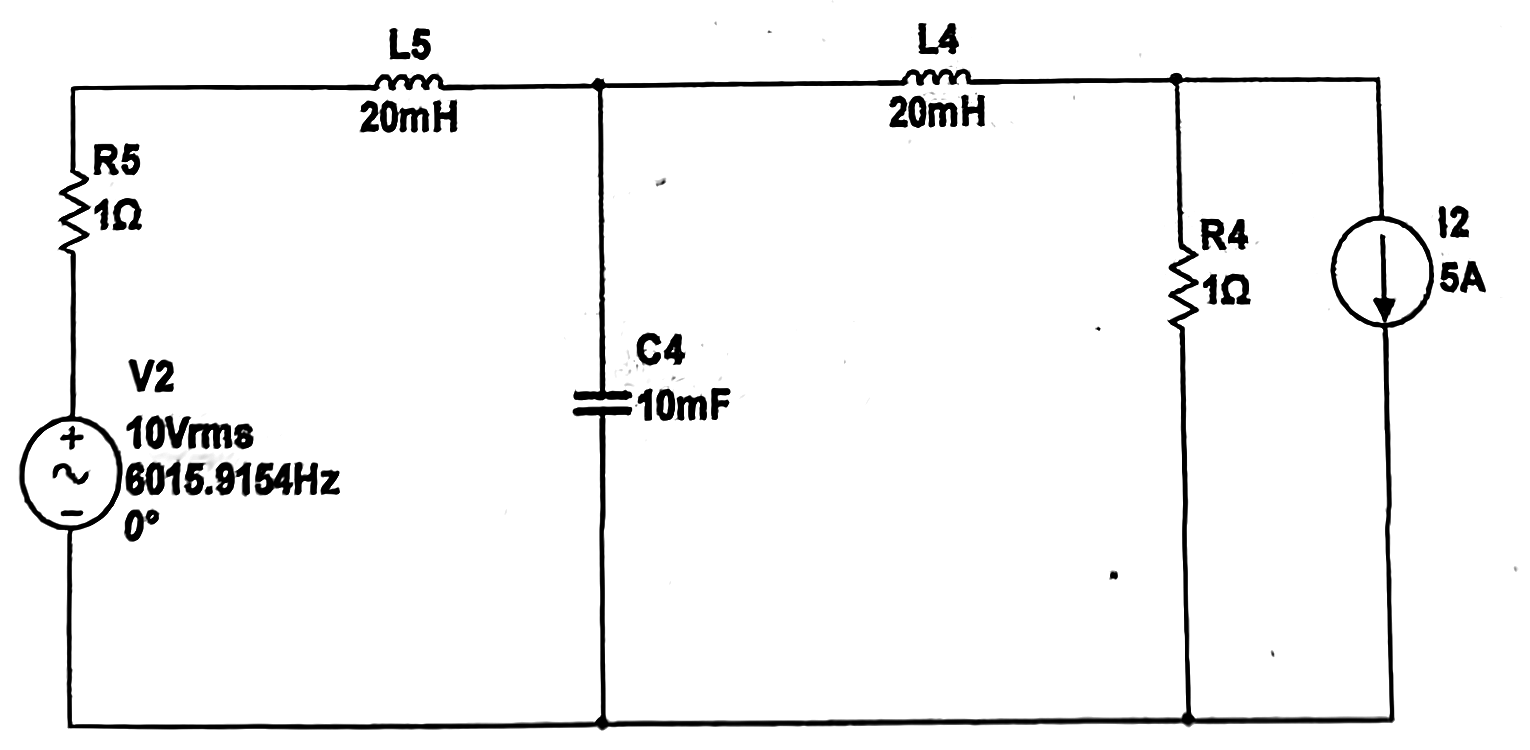
\includegraphics[width=0.8\textwidth]{circuito2.png}
\caption{Circuito 2.}
\label{fig:circuito2}
\end{figure}

Se buscan los fasores $V_k$ y $J_k$ de todas las ramas. Los elementos son $R_4 = R_5 = 1\,\Omega$,
$L_4 = L_5 = 20$~mH y $C_4 = 10$~mF.

\subsection{Desarrollo}

\paso{1. Fuentes reales}

$V_2$ tiene a $R_5$ y $L_5$ en serie e $I_2$ tiene a $R_4$ en paralelo, por lo que las dos fuentes son reales.

\paso{2. Fasores e impedancias}

Las dos fuentes tienen $\omega = 100$~rad/s. Sus fasores son
\[
  V_2 = \pol{2}{0}\ \text{V}, \qquad I_2 = \pol{5}{75} = 1.2941 + j4.8296\ \text{A}.
\]
En el dibujo, la fuente de voltaje dice 10~V\,rms y 6015.9154~Hz, que no corresponde al enunciado; se usan los datos
del enunciado. Las impedancias son
\[
  Z_{L} = j\omega L = j(100)(0.02) = j2\,\Omega, \qquad
  Z_{C_4} = \frac{1}{j\omega C} = \frac{1}{j(100)(0.01)} = \frac{1}{j1} = -j1\,\Omega .
\]

\paso{3. Nodos}

\begin{itemize}
  \item Nodo 1, arriba al centro, donde se unen $L_5$, $C_4$ y $L_4$.
  \item Nodo 2, arriba a la derecha, donde se unen $L_4$, $R_4$ e $I_2$.
  \item Nodo 3, todo el cable de abajo. Es el nodo de referencia.
\end{itemize}

\paso{4. Grafo orientado y mallas}

$V_2$, $R_5$ y $L_5$ van en una sola rama, e $I_2$ en la rama de $R_4$. Resultan las cuatro ramas de la
tabla~\ref{tab:ramas2}, y con $b = 4$ y $n = 3$ hay
\[
  b - n + 1 = 4 - 3 + 1 = 2 \ \text{mallas}.
\]

\begin{table}[H]
\centering
\caption{Ramas del circuito 2.}
\label{tab:ramas2}
\begin{tabular}{cccccc}
\toprule
Rama & Sale $\to$ entra & Elementos & $Z_k$ ($\Omega$) & $V_{sk}$ (V) & $J_{sk}$ (A) \\
\midrule
$b_1$ & $1 \to 3$ & $L_5$, $R_5$ y $V_2$ & $1 + j2$ & $2$ & $0$ \\
$b_2$ & $1 \to 3$ & $C_4$ & $-j1$ & $0$ & $0$ \\
$b_3$ & $1 \to 2$ & $L_4$ & $j2$ & $0$ & $0$ \\
$b_4$ & $2 \to 3$ & $R_4$ e $I_2$ & $1$ & $0$ & $\pol{5}{75}$ \\
\bottomrule
\end{tabular}
\end{table}

Las mallas van en sentido horario: $M_1 = \{b_1, b_2\}$ a la izquierda y $M_2 = \{b_2, b_3, b_4\}$ a la derecha
(figura~\ref{fig:grafo2}).

\begin{figure}[H]
\centering
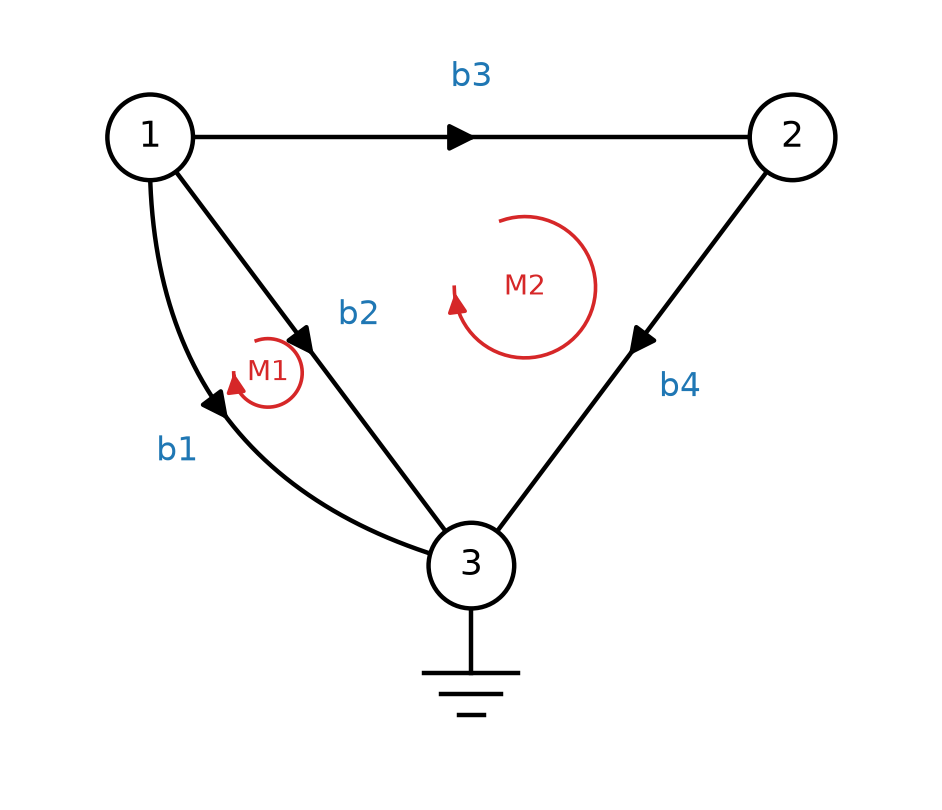
\includegraphics[width=0.6\textwidth]{grafo_circuito2.png}
\caption{Grafo orientado del circuito 2, dibujado por el programa.}
\label{fig:grafo2}
\end{figure}

\paso{5. Matriz de mallas}

$M_1$ sube por $b_1$, que va al revés, y baja por $b_2$, que va en el mismo sentido. $M_2$ sube por $b_2$, que va al
revés, y sigue por $b_3$ y $b_4$, que van en el mismo sentido:
\[
M = \begin{bmatrix}
 -1 &  1 & 0 & 0 \\
  0 & -1 & 1 & 1
\end{bmatrix}.
\]

\paso{6. Matriz de impedancias de rama}

\[
Z = \operatorname{diag}\left(1 + j2,\ -j1,\ j2,\ 1\right)\ \Omega .
\]

\paso{7. Vectores de fuentes}

$b_1$ baja del nodo 1 al 3 y entra a $V_2$ por su terminal $+$, por lo que $V_{s1} = 2$. $b_4$ baja del nodo 2 al 3
y la flecha de $I_2$ también apunta hacia abajo, por lo que $J_{s4} = \pol{5}{75}$:
\[
V_{sk} = \begin{bmatrix} 2 & 0 & 0 & 0 \end{bmatrix}^T \text{V}, \qquad
J_{sk} = \begin{bmatrix} 0 & 0 & 0 & 1.2941 + j4.8296 \end{bmatrix}^T \text{A}.
\]
En el programa son \texttt{valoresExamen2}, \texttt{matrizMallas2} y \texttt{armarCircuito2}, escritos igual que
los del circuito 1.

\paso{8. Matriz de impedancias de mallas}

Las dos mallas comparten $b_2$:
\[
Z_{m11} = (1 + j2) + (-j1) = 1 + j1, \quad
Z_{m22} = -j1 + j2 + 1 = 1 + j1, \quad
Z_{m12} = (1)(-1)(-j1) = j1,
\]
\[
Z_m = M Z M^T = \begin{bmatrix} 1 + j1 & j1 \\ j1 & 1 + j1 \end{bmatrix}
= \begin{bmatrix} \pol{1.4142}{45} & \pol{1}{90} \\ \pol{1}{90} & \pol{1.4142}{45} \end{bmatrix} \Omega .
\]

\paso{9. Potenciales de fuentes independientes de mallas}

$b_1$ tiene $-1$ en $M_1$, por lo que $-M V_{sk}$ aporta $-(-1)(2) = 2$ al primer renglón. $b_4$ tiene $1$ en $M_2$
y $Z_4 J_{s4} = (1)(\pol{5}{75})$, por lo que $M Z J_{sk}$ aporta $\pol{5}{75}$ al segundo:
\[
E_{sm} = M Z J_{sk} - M V_{sk} =
\begin{bmatrix} 2 \\ 1.2941 + j4.8296 \end{bmatrix} =
\begin{bmatrix} \pol{2}{0} \\ \pol{5}{75} \end{bmatrix} \text{V}.
\]

\paso{10. Corrientes de mallas}

Con $I_m = Z_m^{-1} E_{sm}$ el programa da, en amperes,
\begin{lstlisting}[style=salida]
Im = Zm^-1 Esm, corrientes de malla
   1:      1.6483   -2.5907j   =       3.0706 /_   -57.53 grados
   2:      0.9424   +2.2390j   =       2.4292 /_    67.17 grados
\end{lstlisting}

\paso{11. Corrientes de rama}

Con $J_k = M^T I_m$ se obtiene $J_1 = -I_1$, $J_2 = I_1 - I_2$ y $J_3 = J_4 = I_2$, porque $b_3$ y $b_4$ solo son de $M_2$.
El programa da, en amperes,
\begin{lstlisting}[style=salida]
Jk = M^T Im, corrientes de rama
   1:     -1.6483   +2.5907j   =       3.0706 /_   122.47 grados
   2:      0.7059   -4.8296j   =       4.8809 /_   -81.68 grados
   3:      0.9424   +2.2390j   =       2.4292 /_    67.17 grados
   4:      0.9424   +2.2390j   =       2.4292 /_    67.17 grados
\end{lstlisting}

$J_4$ incluye la corriente de $I_2$. La corriente de $R_4$ es
\[
J_4 - J_{s4} = (0.9424 + j2.2390) - (1.2941 + j4.8296) = -0.3517 - j2.5907 = \pol{2.6144}{-97.73}\ \text{A}.
\]

\paso{12. Voltajes de rama}

Con $V_k = V_{sk} + Z J_k - Z J_{sk}$ el programa da, en volts,
\begin{lstlisting}[style=salida]
Vk = Vsk + Z Jk - Z Jsk, voltajes de rama
   1:     -4.8296   -0.7059j   =       4.8809 /_  -171.68 grados
   2:     -4.8296   -0.7059j   =       4.8809 /_  -171.68 grados
   3:     -4.4779   +1.8848j   =       4.8584 /_   157.17 grados
   4:     -0.3517   -2.5907j   =       2.6144 /_   -97.73 grados
\end{lstlisting}
$V_4$ es igual a la corriente de $R_4$ porque $R_4 = 1\,\Omega$.

\paso{Comprobación}

$b_1$ y $b_2$ van entre los mismos nodos, por lo que debe cumplirse $V_1 = V_2$, y así ocurre. En la malla $M_2$ la
suma de voltajes es cero:
\[
-V_2 + V_3 + V_4 = (4.8296 + j0.7059) + (-4.4779 + j1.8848) + (-0.3517 - j2.5907) = 0 .
\]
La comparación con una solución por nodos está en la sección~\ref{sec:pruebas}.

% ===================== PRUEBAS =====================
\clearpage
\section{Pruebas y resultados}
\label{sec:pruebas}

\subsection{Comparación con el método de nodos}

Para comprobar el programa, los dos circuitos se resolvieron también por nodos, con las ramas escritas aparte de las
del programa. Con la matriz de incidencia reducida $A$, sin el renglón del nodo de referencia, y $Y = Z^{-1}$, los
potenciales de nodo $e$ se obtienen de
\[
  A Y A^T e = A Y V_{sk} - A J_{sk},
\]
y de ellos $V_k = A^T e$ y $J_k = Y V_k - Y V_{sk} + J_{sk}$. Además se revisó que los resultados del programa
cumplan la ley de corrientes en cada nodo, $A J_k = 0$, y la ley de voltajes en cada malla, $M V_k = 0$. La
tabla~\ref{tab:pruebas} muestra la diferencia más grande en cada caso; el tercer renglón corresponde a la prueba con
valores cambiados de la sección~\ref{sec:valores}.

\begin{table}[H]
\centering
\caption{Diferencias máximas entre el programa y la comprobación independiente.}
\label{tab:pruebas}
\footnotesize
\setlength{\tabcolsep}{4pt}
\begin{tabular}{lcccc}
\toprule
Caso & $\max\lvert J_k - J_k^{\text{nodos}}\rvert$ (A) & $\max\lvert V_k - V_k^{\text{nodos}}\rvert$ (V)
  & $\max\lvert A J_k\rvert$ (A) & $\max\lvert M V_k\rvert$ (V) \\
\midrule
Circuito 1 & $9.5\times10^{-16}$ & $1.5\times10^{-15}$ & $4.1\times10^{-17}$ & $1.2\times10^{-15}$ \\
Circuito 2 & $1.8\times10^{-15}$ & $1.8\times10^{-15}$ & $0$ & $9.2\times10^{-16}$ \\
Circuito 1, $R_3 = 10\,\Omega$ & $1.1\times10^{-15}$ & $2.0\times10^{-15}$ & $1.4\times10^{-17}$ & $2.0\times10^{-15}$ \\
\bottomrule
\end{tabular}
\end{table}

Todas las diferencias son del orden de $10^{-15}$, que corresponde al error de redondeo de los números de punto
flotante. Los dos métodos dan los mismos resultados, y estos cumplen las dos leyes de Kirchhoff.

\subsection{Valores cambiados}
\label{sec:valores}

En la interfaz se cambió $R_3$ del circuito 1 de $1\,\text{k}\Omega$ a $10\,\Omega$, con los demás valores del examen
(figura~\ref{fig:guivalores}). Se eligió $R_3$ porque con $1\,\text{k}\Omega$ la rama $b_6$ casi no lleva corriente, y
con $10\,\Omega$ su efecto se nota en todo el circuito. La corriente de $b_6$ sube de 2.8~mA a
$\pol{0.2685}{-91.45}$~A y las demás también cambian; por ejemplo, $J_1$ pasa de $\pol{1.3937}{3.16}$ a
$\pol{1.3494}{4.26}$~A. La solución por nodos da los mismos valores (tabla~\ref{tab:pruebas}).

\begin{figure}[H]
\centering
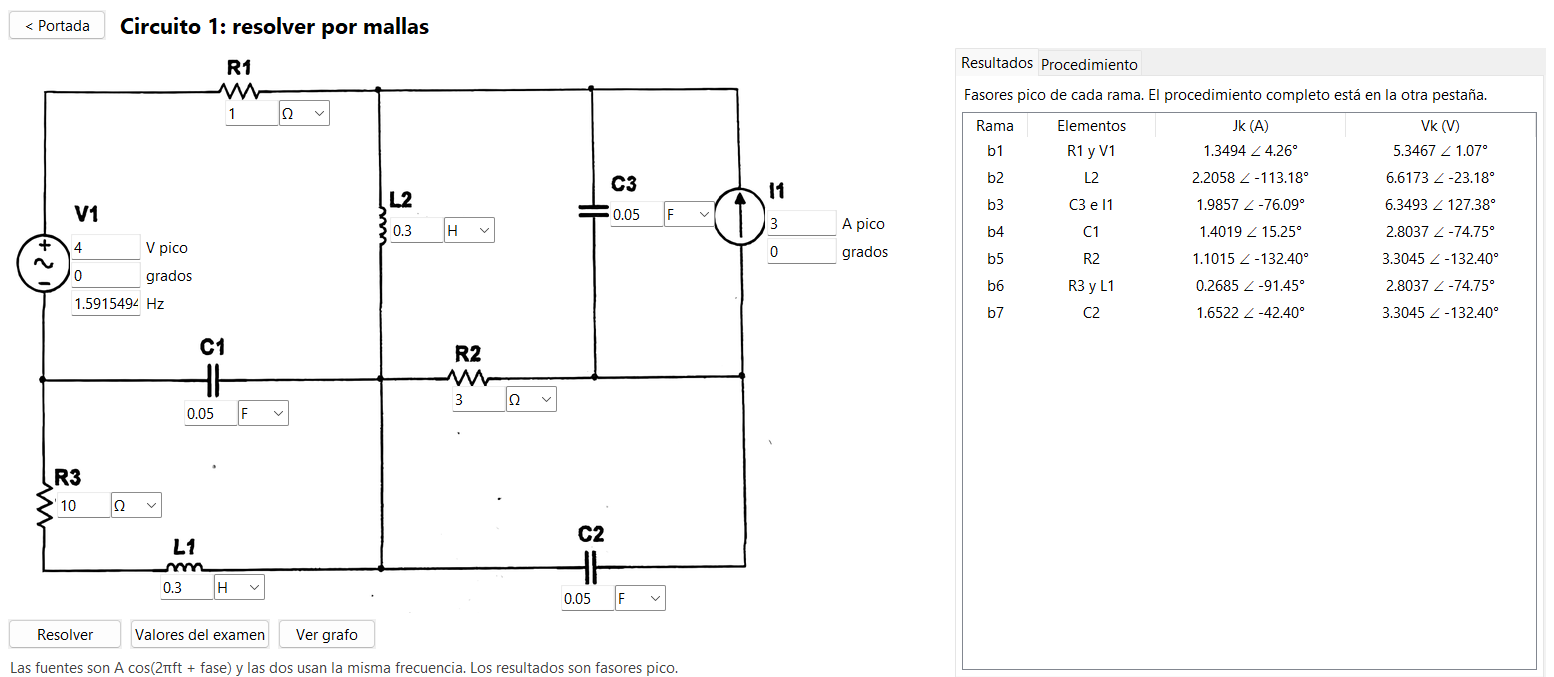
\includegraphics[width=\textwidth]{gui_valores_cambiados.png}
\caption{Circuito 1 con $R_3 = 10\,\Omega$.}
\label{fig:guivalores}
\end{figure}

\subsection{Valores no válidos}

La interfaz revisa los valores antes de resolver. Si una casilla está vacía o no tiene un número, si un valor es
negativo, excepto las fases, si un capacitor o la frecuencia valen cero, o si con esos valores $Z_m$ no tiene inversa,
no resuelve y muestra un mensaje que pide cambiar los valores (figura~\ref{fig:guierror}).

\begin{figure}[H]
\centering
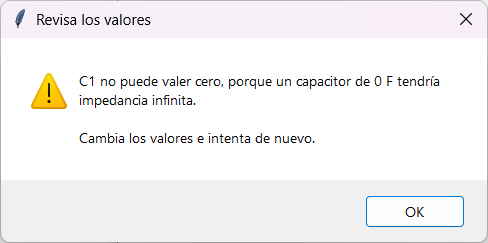
\includegraphics[width=0.5\textwidth]{gui_error.png}
\caption{Mensaje con $C_1 = 0$.}
\label{fig:guierror}
\end{figure}

% ===================== CONCLUSIONES =====================
\clearpage
\section{Conclusiones}

Esperábamos que lo difícil fueran las cuentas con números complejos, pero el programa las hace en una línea por paso.
Lo que más tuvimos que pensar fue el grafo, sobre todo qué elementos van juntos en una rama. El circuito 1 tiene once
elementos, y al juntar $V_1$ con $R_1$, $R_3$ con $L_1$ y poner $I_1$ en la rama de $C_3$ resultaron siete ramas y
cuatro mallas. Con cada elemento en su propia rama habríamos tenido más mallas sin necesidad.

Un problema fue interpretar bien las corrientes de las ramas con fuente de corriente. La $J_3$ que da el programa es la
de toda la rama, no la de $C_3$; la de $C_3$ se obtiene de $J_3 - J_{s3}$. Con $R_4$ e $I_2$ ocurre lo mismo. También
nos llamó la atención que por $b_6$ pasaran solo 2.8~mA. Es correcto, porque $R_3 = 1\,\text{k}\Omega$ está en paralelo
con un capacitor de $2\,\Omega$, y la prueba con $R_3 = 10\,\Omega$ mostró que la corriente de esa rama crece cuando
$R_3$ baja. En el circuito 2, los datos de la fuente en el dibujo no coinciden con el enunciado, y usamos los del
enunciado.

Como $M$ se escribe a mano, hicimos que el programa la revise contra la matriz de incidencia antes de resolver, para que
un signo equivocado no pase sin aviso. Además comparamos los resultados con una solución por nodos y con las leyes de
Kirchhoff, también con valores distintos a los del examen, y las diferencias fueron solo de redondeo. Que el programa
muestre cada matriz en el orden del procedimiento nos sirvió para comparar cada paso con lo que hicimos a mano.

En la segunda versión agregamos una interfaz gráfica para cambiar los valores de los elementos y de las fuentes. La
hicimos aparte del código del método. La interfaz solo lee los valores y llama a las mismas funciones que la versión
de terminal, de modo que el cálculo sigue siendo igual de fácil de explicar paso por paso. Para que la interfaz pudiera
cambiar los valores, los datos de cada circuito pasaron a ser una función que los recibe. Las revisiones de los valores de entrada las dejamos en lo mínimo, e
incluyen el caso en que $Z_m$ no tiene inversa, que la primera versión no trataba.

El método matricial ya resolvía la parte de las cuentas, porque una vez que se tienen $M$, $Z$, $V_{sk}$ y $J_{sk}$,
los pasos 8 a 12 son siempre los mismos. Lo que tuvimos que hacer fue interpretar cada circuito y escribir bien esos datos, y las
pruebas nos mostraron que los errores posibles están en esa parte y no en el cálculo.

\end{document}
